\chapter{Comparison of Available Datasets}
\label{sec:dataset_selection}

This chapter builds upon the insights elaborated in previous chapters to lay the foundation
for developing a classifier for the \cgls{3L-CVRP} with practical constraints by comparing and
selecting a suitable dataset. The classifier will be used to predict the feasibility of packing a
given set of cuboids into a vehicle - representing a single tour - similar to the approach presented
in Chapter~\ref{sec:motivation_feasibility_prediction} by \citeauthor*{zhang_learning-based_2022}.
As discussed in Chapter~\ref{sec:classical_solution_approaches}, the \gls{CLP} is an NP-hard problem,
making it computationally demanding to verify the packing feasibility of individual routes.
A classifier can therefore enhance the performance of existing exact algorithms\footcite[cf.][]{tamke_branch-and-cut_2024} by reducing the need to compute feasibility exactly - using \cgls{CP} methods - only when a final solution is found, or just before columns generated in Branch-and-Price or Branch-and-Cut algorithms are discarded \footcite[cf.][pp. 9--11]{zhang_learning-based_2022}. As many single routes need to be evaluated, this use case has the potential to significantly reduce the overall
computation time. First, five published \cgls{3L-CVRP} datasets will be compared with respect
to their overall characteristics. Subsequently, a more detailed analysis will focus on the
heterogeneity of the items. Finally, a suitable dataset will be selected as a promising foundation
for developing a classifier.

The first \cgls{3L-CVRP} dataset was published by \citeauthor*{gendreau_tabu_2006} in
\citeyear{gendreau_tabu_2006} and delivered the first \cgls{3L-CVRP} instances.
The second dataset was published by \citeauthor*{moura_integrated_2009} in \citeyear{moura_integrated_2009}, and combines the Solomon benchmark instances\footcite[cf.][]{solomon_algorithms_1987} and the \gls{CLP} instances from \citeauthor*{bischoff_issues_1995} defining the \gls{3L-VRPTW}. \citeauthor*{ceschia_local_2013} published a \cgls{3L-CVRP} dataset in \citeyear{ceschia_local_2013} representing real-life data and \citeauthor*{krebs_advanced_2021} published two different datasets in \citeyear{krebs_advanced_2021} with a focus on more realistic constraints. The characteristics of the single different datasets are summarized in the follwing Table~\ref{tab:dataset_comparison}. It needs to be noted, that all instances consider either the \cgls{3L-CVRP} or the \cgls{3L-VRPTW}.

\clearpage
\begin{table}[h]
    \centering
    \small
    \begin{tabular}{@{}lcccc@{}}
        \toprule
        \textbf{Reference}                                  & \textbf{Instances} & \textbf{Customers}  & \textbf{Rel. Mass Range} & \textbf{Orders Range}   \\
        \midrule
        Gendreau, 2006\footcite[cf.][]{gendreau_tabu_2006}  & 27                 & [15, 100]           & [0, 0.91]                & [1, 3]                  \\
        Moura, 2009\footcite[cf.][]{moura_integrated_2009}  & 46                 & 25                  & [0, 0.01]                & [30, 100]               \\
        Ceschia, 2013\footcite[cf.][]{ceschia_local_2013}   & 13                 & [11, 129]           & [0, 0.05]                & [1, 41]                 \\
        Krebs\_a, 2021\footcite[cf.][]{krebs_advanced_2021} & 600                & 20, 60, 100         & [0, 0.58]                & [1, 30]                 \\
        Krebs\_b, 2021\footcite[cf.][]{krebs_axle_2021}     & 80                 & 30, 60, 90, 120     & [0, 0.04]                & [1, 22]                 \\
        \toprule
        \textbf{Reference}                                  & \textbf{Items}     & \textbf{Item Types} & \textbf{Min dimension}   & \textbf{Max dimensions} \\
        \midrule
        Gendreau, 2006                                      & [26, 199]          & [26, 199]           & \{12, 5, 6\}             & \{36, 15, 18\}          \\
        Moura, 2009                                         & 1050, 1550         & 5                   & \{8.1, 3.3, 2.5\}        & \{12, 9.9, 7.3\}        \\
        Ceschia, 2013                                       & [254, 8060]        & [9, 97]             & \{0.1, 0.5, 0.1\}        & \{66, 23, 28.4\}        \\
        Krebs\_a, 2021                                      & 200, 400           & 3, 10, 100          & \{6, 2, 2\}              & \{35, 14, 14\}          \\
        Krebs\_b, 2021                                      & 200, 400           & 10, 100             & \{6, 6, 6\}              & \{25, 12, 15\}          \\
        \bottomrule
    \end{tabular}
    \caption{Numeric comparisons between available datasets.}
    \label{tab:dataset_comparison}
\end{table}
\begin{comment}
\begin{table}[!ht]
    \centering
    \small
    \begin{tabular}{@{}lcccc@{}}
        \toprule
        \textbf{Reference}                                  & \textbf{Instances} & \textbf{Customers}  & \textbf{Rel. Mass Range} & \textbf{Orders Range}   \\
        \midrule
        Gendreau, 2006\footcite[cf.][]{gendreau_tabu_2006}  & 27                 & [15, 100]           & [0, 0.91]                & [1, 3]                  \\
        Moura, 2009\footcite[cf.][]{moura_integrated_2009}  & 46                 & 25                  & [0, 0.01]                & [30, 100]               \\
        Ceschia, 2013\footcite[cf.][]{ceschia_local_2013}   & 13                 & [11, 129]           & [0, 0.05]                & [1, 41]                 \\
        Krebs\_a, 2021\footcite[cf.][]{krebs_advanced_2021} & 600                & \{20, 60, 100\}     & [0, 0.58]                & [1, 30]                 \\
        Krebs\_b, 2021\footcite[cf.][]{krebs_axle_2021}     & 80                 & \{30, 60, 90, 120\} & [0, 0.04]                & [1, 22]                 \\
        \toprule
        \textbf{Reference}                                  & \textbf{Items}     & \textbf{Item Types} & \textbf{Min dimension}   & \textbf{Max dimensions} \\
        \midrule
        Gendreau, 2006                                      & [26, 199]          & [26, 199]           & \{12, 5, 6\}             & \{36, 15, 18\}          \\
        Moura, 2009                                         & \{1050, 1550\}     & 5                   & \{8.1, 3.3, 2.5\}        & \{12, 9.9, 7.3\}        \\
        Ceschia, 2013                                       & [254, 8060]        & [9, 97]             & \{0.1, 0.5, 0.1\}        & \{66, 23, 28.4\}        \\
        Krebs\_a, 2021                                      & \{200, 400\}       & \{3, 10, 100\}      & \{6, 2, 2\}              & \{35, 14, 14\}          \\
        Krebs\_b, 2021                                      & \{200, 400\}       & \{10, 100\}         & \{6, 6, 6\}              & \{25, 12, 15\}          \\
        \bottomrule
    \end{tabular}
    \caption{Numeric comparisons between available datasets.}
    \label{tab:dataset_comparison}
\end{table}
\end{comment}

The brackets [\,] indicate a range of possible values, whereas $\{\,\}$ symbolizes tuples and all integers single values. The table summarizes the numerical characteristics of the datasets and differences can easily be identified. Two definitions are important for understanding the overview.
Firstly, “relative” refers to the ratio of item weight to vehicle capacity or dimensions, as the datasets differ and cannot be directly compared and secondly, a item type is defined by its geometrical dimensions, the weight, and possible stability characteristics, such as fragility. It needs to be noted,
that items with the equal type occur multiple times, if the number of item typs is smaller than the
number of items, as in thhe Moura dataset. The relative mass of items differs and the number of ordered
items per customer varies significantly. The Gendreau dataset has the greatest relative mass range, but
the minimum number of requested items per customer.

\begin{table}[h]
    \centering
    \small
    \begin{tabular}{@{}lp{0.8\textwidth}@{}}
        \toprule
        \textbf{Dataset} & \textbf{Constraints}                                                                                                     \\
        \midrule
        Gendreau, 2006   & Rotation, Support, Fragility, LIFO, Sequence                                                                             \\
        Moura, 2009      & TW, LIFO Unloading, Orientation, Cargo stability                                                                         \\
        Ceschia, 2013    & \textit{Load Bearing Strength}, Vertical orientation, \textit{Robust Stability}, \textit{Reachability}                   \\
        Krebs, 2021a     & Vertical orientation, Load-bearing strength, Robust stability, Reachability, Axle weights, balanced loading, manual LIFO \\
        Krebs, 2021b     & Vertical orientation, Axle weights, Fragility, Minimal supporting area, LIFO                                             \\
        \bottomrule
    \end{tabular}
    \caption{Overview of considered constraints of published datasets.}
    \label{tab:constraints_cvrp_instances}
\end{table}

The second table provides an overview of the constraints considered in each paper. All fundamental \gls{CLP} constraints are included, with additional constraints defined in Chapter~\ref{sec:clp_definition}.
The only newly introduced constraint is time windows (TW), which specify the time intervals during which customers can be serviced, adding an additional layer of complexity to the problem.
To further investigate the differences between the datasets, the following Figure~\ref{fig:dataset_comparison}
visualizes the relative mass and volume in comparison to the vehicle volume of all items
requested by single customers of instances in each dataset representing the unconstrained \gls{LB}
on vehicle usage. Additionally the size of the points indicates the aggregated quantity of items.
As an example, the dataset Moura contains 46 instances with 25 customers per instance,
so in this plot the aggregated demands of $25\cdot46= 1115$ customers are shown.

\begin{figure}[h]
    \centering
    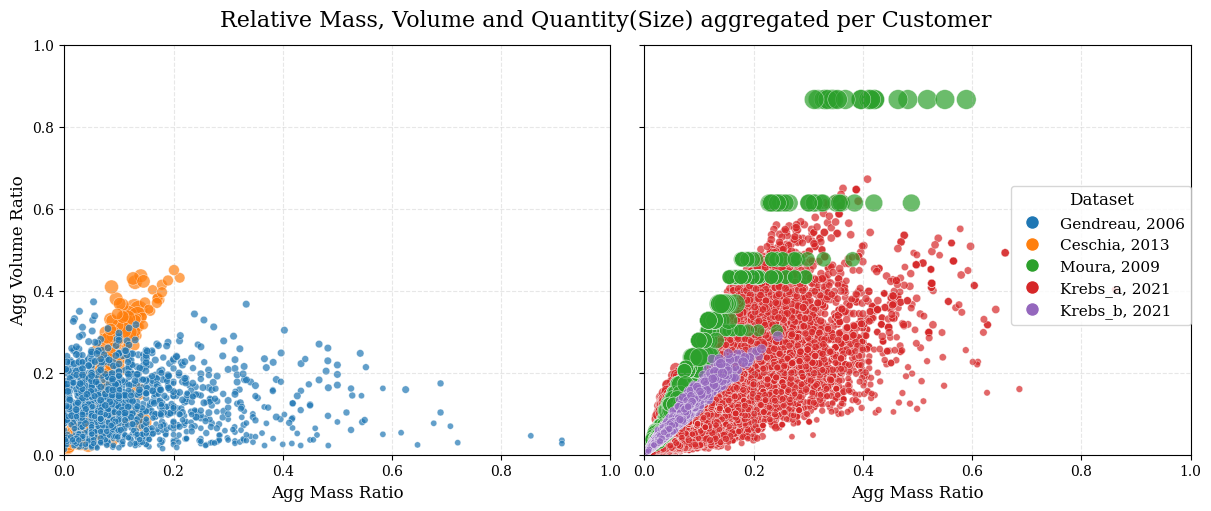
\includegraphics[width=0.8\textwidth]{pictures/comparison_datasets_3lcvrp.png}
    \caption{Comparison of 3L-CVRP/ 3L-VRPTW datasets.}.
    \label{fig:dataset_comparison}
\end{figure}


The dispersion of the data points reflects the diversity of individual instances in terms of volume
and mass dependency. A more balanced profile suggests that some customers tend to order items that
are either mass- or volume-intensive, which supports training the model on more heterogeneous data.
Therefore, the dataset should cover a wide range of cases, varying in mass, volume, and item
quantity per customer. The widest spread is observed in Krebs\_a and Gendreau datasets serving
both as good dataset candidates for training a classifier. However, as depicted in Table~\ref{tab:dataset_comparison},
the items of Gendreau are quite big and the number of deliviered items per customer is with a range
of [1,3] quite small. Consequently, the Krebs\_a dataset is selected as the most suitable and the properties of this dataset will be further investigated.
\clearpage
The dataset Krebs\_a contains 18 different
instance types resulting from the combinations of number of customers, item tyes and items. The following Figure~\ref{fig:krebs_dataset_analysis} shows the distribution of the volume of single instance types of the dataset. It can be clearly seen, that the volume of the items for the instance types with 20 customers is significantly lower than for the instances with 60 or 100 customers.

\begin{figure}[h]
    \centering
    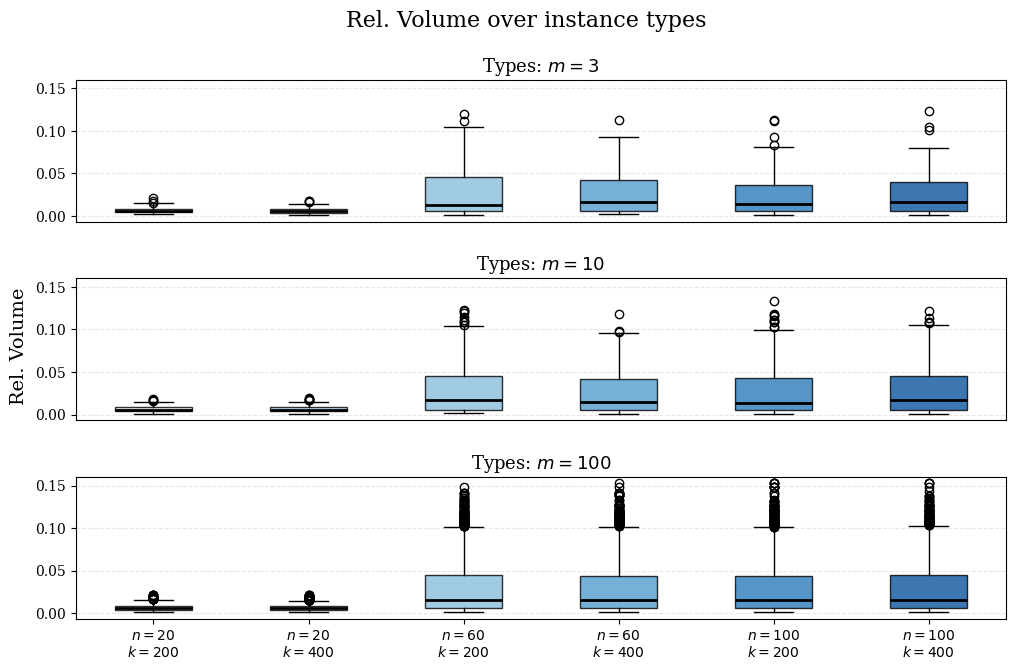
\includegraphics[width=0.6\textwidth]{pictures/volume_over_instances_krebs.png}
    \caption[Visualization of volume distribution in Krebs et al. (2021) dataset.]{Visualization of volume distribution in Krebs\_a datset.}.
    \label{fig:krebs_dataset_analysis}
\end{figure}

Furthermore, it is interesting to split Figure~\ref{fig:dataset_comparison} into the single 18 instances
of Krebs\_a to identify the heterogeneity of single instance types more in detail. It can be seen, that
the customers demands differ between the single 18 distributions and this needs to be considered, when
generating the training data for the classifier.

\begin{figure}[h]
    \centering
    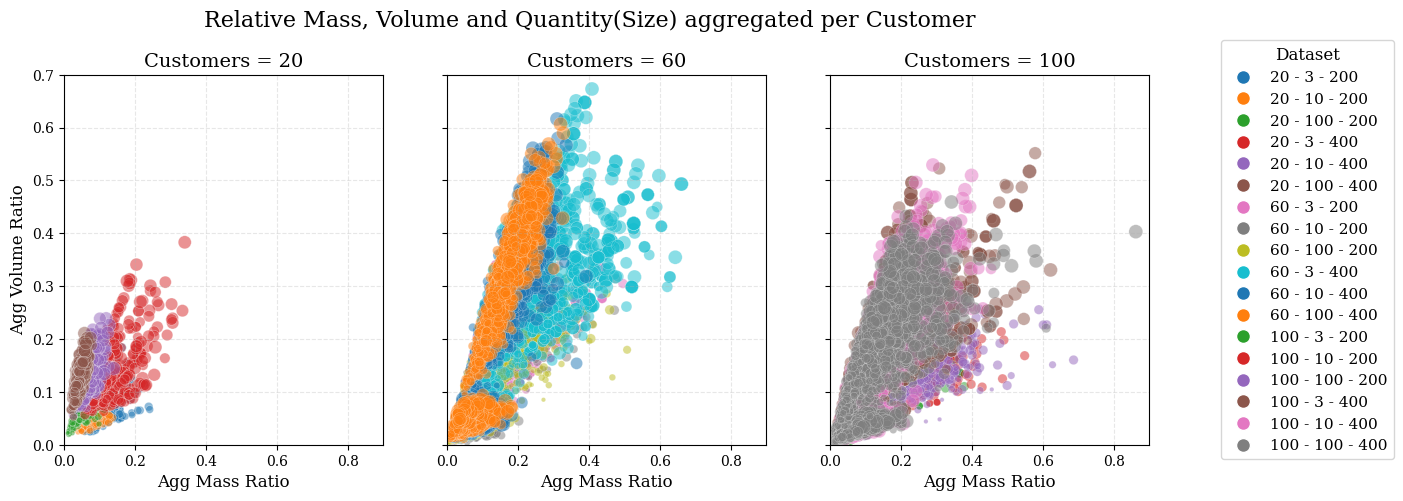
\includegraphics[width=0.9\textwidth]{pictures/krebs_instances_detailed.png}
    \caption[Visualization of different instances of Krebs et al. (2021) dataset.]{Visualization of different instances of Krebs\_a dataset.}.
    \label{fig:krebs_dataset_analysis_detailes}
\end{figure}



%\section{Overview of Public Datasets}
%\section{Evaluation Criteria: Diversity, Realism, Labeling, Size}
%\section{Comparison of Selected Datasets}
%\section{Justification for Dataset Selection}